\documentclass[10pt,oneside]{scrartcl} 
%\documentclass[a4paper,10pt]{article}

\textwidth17cm \textheight24.0cm \topmargin-2.1cm
\evensidemargin-0.5cm \oddsidemargin-0.5cm \parindent0.0cm
\unitlength1.0mm

\usepackage{graphicx}
\usepackage[sort, comma]{natbib}
\usepackage{textcomp}
\usepackage{hyperref}
\usepackage{listings}
\usepackage{color}
\usepackage[utf8]{inputenc}
\usepackage{amsmath}
\usepackage{amssymb} 
\usepackage{algorithm}
\usepackage{algorithmic}

\usepackage{url}
\urlstyle{sf}

\definecolor{blancCasse}{rgb}{0.97,0.88,0.78}
\definecolor{rouge}{rgb}{1.0,0.0,0.0}
\newcommand{\centier}{\left[\hspace{-1ex}\right.\left[\hspace{0.5ex}\right.}
\newcommand{\oentier}{\left]\hspace{-1ex}\right.\left]\hspace{0.5ex}\right.}

\newcommand\vecteur[1]{\boldsymbol#1}
\newcommand\matrice[1]{\mathbf#1}
\newcommand\trace{\operatorname*{Tr}}
\newcommand\cov{\operatorname*{cov}}

%[[ = \left[\hspace{-1ex}\left[\hspace{0.5ex} ; ou \left[\kern-0.15em\left[
%]] = \hspace{0.5ex} \right]\hspace{-1ex}\right]} ; ou \right]\kern-0.15em\right] }

%\usepackage{amsmath}
%opening
\title{An introduction to Kalman filters}
\author{Jeremy Fix}

\begin{document}

\maketitle

\tableofcontents

\pagebreak

\section{Preliminaries}
\label{sec_kalman_math}
\subsection{Notation}

In the following, we denote $x$ a scalar, $\vecteur{x}$ a vector and $\matrice{X}$ a matrix. Vectors are supposed to be column vectors, i.e. $\vecteur{x}^T\vecteur{y}$ is the scalar product between $\vecteur{x}$ and $\vecteur{y}$.We denote $A_{i,j}$ the component at row $i$, column $j$ of a matrix $\matrice{A}$. The trace of a matrix $A \in M(n,m)$ equals : $\trace(A) = \sum_{i=1}^{min(n,m)} A_{ii}$. \\

\subsection{Matrix derivative}

The derivation of a matrix $A$ according to a matrix $X$ (it equals zero if $A$ is not an expression depending on $X$) reads :
\begin{eqnarray}
\frac{\partial \matrice{A}}{\partial \matrice{X}} =\begin{bmatrix}
\frac{\partial\mathbf{A}}{\partial X_{1,1}} & \cdots & \frac{\partial \mathbf{A}}{\partial X_{1,m}}\\
\vdots & \ddots & \vdots\\
\frac{\partial\mathbf{A}}{\partial X_{n,1}} & \cdots & \frac{\partial \mathbf{A}}{\partial X_{n,m}}\\
\end{bmatrix}
\end{eqnarray}
We can then demonstrate the following identities :
\begin{eqnarray}
\frac{d \trace(\matrice{A} \matrice{C})}{d \matrice{A}} &=& \begin{bmatrix}
\frac{\partial \sum_i \sum_k \matrice{A}_{i,k}\matrice{C}_{k,i}}{\partial A_{1,1}} & \cdots & \frac{\partial \sum_i \sum_k A_{i,k}C_{k,i}}{\partial A_{1,m}}\\
\vdots & \ddots & \vdots\\
\frac{\partial\sum_i \sum_k A_{i,k}C_{k,i}}{\partial A_{n,1}} & \cdots & \frac{\partial \sum_i \sum_k A_{i,k}C_{k,i}}{\partial A_{n,m}}
\end{bmatrix}
= \begin{bmatrix}
C_{1,1} & \cdots & C_{m,1}\\
\vdots & \ddots & \vdots\\
C_{1,n} & \cdots & C_{m,n}
\end{bmatrix}
= \matrice{C}^T\\
\frac{d \trace(\matrice{A} \matrice{B} \matrice{A}^T)}{d\matrice A} &=& \matrice{A}\matrice{B} + \matrice{A}\matrice{B}^T \\ 
                                                                    &=& 2 \matrice{A} \matrice{B},\mbox{ if } \matrice{B} \mbox{ is symmetric}
\end{eqnarray} 

\subsection{Variance/covariance of random vectors}

The covariance matrix of a random vector $\vecteur{x}$ is defined as :
\begin{eqnarray}
\nonumber \cov(\vecteur{x}) = E[(\vecteur{x} - E[\vecteur{x}]).(\vecteur{x} - E[\vecteur{x}])^T]
\end{eqnarray}

If $\vecteur{x}$ and $\vecteur{y}$ are random vectors, their covariance is defined as :
\begin{eqnarray}
\nonumber \cov(\vecteur{x},\vecteur{y}) &=& E[(\vecteur{x} - E[\vecteur{x}]).(\vecteur{y} - E[\vecteur{y}])^T]\\
\nonumber                               &=& \cov(\vecteur{y}, \vecteur{x})^T
\end{eqnarray}

The covariance of the sum of two random vectors $\vecteur{x},\vecteur{y}$ reads :
\begin{eqnarray}
\nonumber \cov(\vecteur{x} + \vecteur{y}) = \cov(\vecteur{x}) + \cov(\vecteur{x},\vecteur{y}) + \cov(\vecteur{y},\vecteur{x}) + \cov(\vecteur{y}) 
\end{eqnarray}

By definition, if the two random vectors are independent, then $\cov(\vecteur{x}, \vecteur{y}) = 0$. Therefore, the covariance matrix of the sum $\vecteur{x}+\vecteur{y}$ of two independent random vectors $\vecteur{x}$ and $\vecteur{y}$ equals the sum of the covariance matrix of the two vectors :
\begin{eqnarray}
\label{eq:preliminaries_esperance_independent} \mbox{If $\vecteur{x}$ and $\vecteur{y}$ are independent}, \cov(\vecteur{x} + \vecteur{y}) = \cov(\vecteur{x})+\cov(\vecteur{y})
\end{eqnarray}
The covariance of a linear transformation of random vector $\vecteur{x}$ reads : 
\begin{eqnarray}
\nonumber \cov(\matrice{A} \vecteur{x}) = \matrice{A}\cov(\vecteur{x})\matrice{A}^T
\end{eqnarray}
Finally, for $\vecteur{x_1},\vecteur{x_2},\vecteur{y}$ three random vectors, we have the identity :
\begin{eqnarray}
\nonumber \cov(\vecteur{x_1} + \vecteur{x_2}, \vecteur{y}) = \cov(\vecteur{x_1},\vecteur{y}) + \cov(\vecteur{x_2},\vecteur{y})
\end{eqnarray}
\subsection{Assumptions behind kalman filtering}

\textcolor{red}{Todo}

- The whiteness of noise\\
- only the first and second order moments are propagated\\

\section{Discrete Kalman filter with linear state-space formulation}

The presentation below follows \cite{Welch2006}. Consider a state $x_k
\in \mathbb{R}^n$ for which we get an observation $y_k \in
\mathbb{R}^m$, the state evolving according to a linear recursive
equation under the influence of an external input $u_k$ and the observations being linearly linked to the state :
\begin{eqnarray}
\vecteur{x_k} &=& \matrice{A}_k \vecteur{x}_{k-1} + \matrice{B}_k
\vecteur{u}_k + \vecteur{w}_{k}\\
\label{kalman_state_space} \vecteur{y_k} &=& \matrice{H}_k \vecteur{x_k} + \vecteur{v_k}
\end{eqnarray}
the evolution and observation being subject to some white and independent noises $w_k,v_k$. In addition to be zero-mean, these noises are supposed to be normally distributed with a variance/covariance matrix denoted respectively $Q_k$ and $R_k$ : $w_k\sim N(0,Q_k), v_k \sim N(0,R_k)$\\

Kalman filtering seeks to get the best estimate of the state $x_k$ given the observations $y_k$, starting from an initial estimate $\hat{x}_0$, the uncertainty on this prior estimate $P_0$, and using a linear update of the form : $\hat{x}_k = \hat{x}_{k-1} + K (y_k - H \hat{x}_{k-1})$.\\

Let's denote the a priori estimate of the state $\hat{x}^-_k$ and the a posteriori estimate of the state $\hat{x}_k$. Let's denote $e^-_k$ and $e_k$ respectively the a priori and the a posteriori errors, and $P_k^-,P_k$ their respective covariances :
\begin{eqnarray}
\nonumber e^-_k &=& x_k - \hat{x}^-_k\\
\nonumber P_k^- &=& E[e^-_k {e^-_k}^T]\\
\nonumber e_k &=& x_k - \hat{x}_k\\
\label{eq_kalman_posterior_error} P_k &=& E[e_k e_k^T] %= 1/k \sum_{i=0}^{k-1} e_i e_i^T
\end{eqnarray}
The problem is to derive the expression of the Kalman gain that allows to get a linear update of an a priori estimate with the difference between the observation and a predicted observation and minimizing the a posteriori error on all the components of the state i.e. the trace of the covariance $e_k^T e_k = \trace(P_k)$. 


\subsection{Prediction}

The first step of the Kalman filter is to predict the state, its covariance as well as the observations. It will be followed by a correction step which seeks to correct our estimate of the state given the discrepancy between the predicted observation and the real observation. Given an estimation of the state $\hat{\vecteur{x}}_{k-1}$ and its associated covariance $\matrice{P_{k-1}}$, a prediction of the state at time $k$ is defined as :
\begin{eqnarray}
\hat{\vecteur{x}}^-_k &=& \matrice{A}_k \hat{\vecteur{x}}_{k-1} + \matrice{B}_k \vecteur{u}_k
\end{eqnarray}

Given this prediction, we can compute its associated covariance using
the evolution equation :
\begin{eqnarray}
\matrice{P_{k-1}}^- &=& E[\vecteur{e_k}^- \vecteur{e_k}^{-T}] = E[(\vecteur{x}_k - \hat{\vecteur{x}}_k^-).(\vecteur{x}_k - \hat{\vecteur{x}}_k^-)^T]\\
                  &=& E[(\vecteur{x}_k - \matrice{A}_k
  \hat{\vecteur{x}}_{k-1} - \matrice{B}_k
  \vecteur{u}_k).(\vecteur{x}_k - \matrice{A}_k
  \hat{\vecteur{x}}_{k-1} - \matrice{B}_k \vecteur{u}_k)^T]\\
\label{eq:kalman_prediction_1}                  &=& E[(\matrice{A}_k
  \vecteur{x}_{k-1} + \matrice{B}_k \vecteur{u}_k + \vecteur{w}_{k} -
  \matrice{A}_k \hat{\vecteur{x}}_{k-1} - \matrice{B}_k \vecteur{u}_k).(\matrice{A}_k\vecteur{x}_{k-1} +
  \matrice{B}_k \vecteur{u}_k + \vecteur{w}_k - \matrice{A} \hat{\vecteur{x}}_{k-1}- \matrice{B}_k \vecteur{u}_k)^T]\\
\label{eq:kalman_prediction_2}                  &=& E[\matrice{A}_k (\vecteur{x}_{k-1} + \hat{\vecteur{x}}_{k-1}).(\vecteur{x}_{k-1} + \hat{\vecteur{x}}_{k-1})^T \matrice{A}_k^T] + E[\vecteur{w}_k \vecteur{w}_k^T] \\
                  &=& \matrice{A}_k \matrice{P}_{k-1} \matrice{A}_k^T + \matrice{Q}_k
\end{eqnarray}

From equation (\ref{eq:kalman_prediction_1}) to equation (\ref{eq:kalman_prediction_2}), we make use of the identity (\ref{eq:preliminaries_esperance_independent}) since $\matrice{A}(\vecteur{x}_{k-1}+\hat{\vecteur{x}}_{k-1})$ and $\vecteur{w}_k$ are independent.

\subsection{Correction}

Given our prediction of the state, its covariance and the associated observations, we now want to linearly correct these estimates. Therefore we want to derive the expression of the Kalman gain $\matrice{K_k}$ such that the correction $\hat{\vecteur{x}}_k = \hat{\vecteur{x}}_k^- + \matrice{K}_k (\vecteur{y}_k - \matrice{H} \hat{\vecteur{x}}_k^-)$ minimizes the a posterior error made on each component of the state. The expression (\ref{eq_kalman_posterior_error}) can be expanded using the equations (\ref{kalman_state_space}): 
\begin{eqnarray}
\nonumber \matrice{P_k} &=& E[\vecteur{e}_k \vecteur{e}_k^T] = E[(\vecteur{x}_k - \hat{\vecteur{x}}_k)(\vecteur{x}_k - \hat{\vecteur{x}}_k)^T]\\
\nonumber     &=& E[(\vecteur{x}_k - (\hat{\vecteur{x}}^-_k + \matrice{K}_k (\vecteur{y}_k - \matrice{H}_k \hat{\vecteur{x}}^-_k)))(\vecteur{x}_k - (\hat{\vecteur{x}}^-_k + \matrice{K}_k (\vecteur{y}_k - \matrice{H}_k \hat{\vecteur{x}}^-_k)))^T]\\
\nonumber     &=& E[(\vecteur{x}_k - (\hat{\vecteur{x}}^-_k + \matrice{K}_k (\matrice{H}_k \vecteur{x}_k + \vecteur{v}_k - \matrice{H}_k \hat{\vecteur{x}}^-_k)))(\vecteur{x}_k - (\hat{\vecteur{x}}^-_k + \matrice{K}_k (\matrice{H}_k \vecteur{x}_k + \vecteur{v}_k - \matrice{H}_k \hat{\vecteur{x}}^-_k)))^T]\\
\nonumber     &=& E[((\matrice{I} - \matrice{K_k} \matrice{H}_k)(\vecteur{x_k} - \hat{\vecteur{x}}^-_k) - \matrice{K_k} \vecteur{v_k})((\matrice{I} - \matrice{K_k} \matrice{H}_k)(\vecteur{x_k} - \hat{\vecteur{x}}^-_k) - \matrice{K_k} \vecteur{v_k})^T]\\
\end{eqnarray}

Given the noise $w$ is white and independent, we can simplify the previous equation :
\begin{eqnarray}
\nonumber \matrice{P_k} &=& E[((\matrice{I} - \matrice{K_k} \matrice{H}_k)(\vecteur{x_k} - \hat{\vecteur{x}}^-_k))((\matrice{I} - \matrice{K_k} \matrice{H}_k)(\vecteur{x_k} - \hat{\vecteur{x}}^-_k))^T] + E[(K_k v_k)(K_k v_k)^T]\\
\nonumber &=& (\matrice{I} - \matrice{K_k} \matrice{H}_k).E[(\vecteur{x_k} - \hat{\vecteur{x}}^-_k))(\vecteur{x_k} - \hat{\vecteur{x}}^-_k))^T].(\matrice{I} - \matrice{K_k} \matrice{H}_k)^T + \matrice{K_k} E[\vecteur{v_k} \vecteur{v_k}^T] \matrice{K_k}^T \\
\label{joseph_form} &=& (\matrice{I} - \matrice{K_k} \matrice{H}) \matrice{P^-_k} (\matrice{I} - \matrice{K_k} \matrice{H})^T + \matrice{K_k} \matrice{R_k} \matrice{K_k}^T \\
\label{eq_kalman_estimate_cov} &=& \matrice{P^-_k} + (\matrice{K_k} \matrice{H}_k \matrice{P^-_k} \matrice{H}_k^T \matrice{K_k}^T) - \matrice{K_k} \matrice{H}_k \matrice{P^-_k} - \matrice{P^-_k} \matrice{H}_k^T \matrice{K_k}^T +  \matrice{K_k} \matrice{R_k} \matrice{K_k}^T
\end{eqnarray}

The equation \ref{joseph_form} is known as the Joseph form of the covariance update equation. As we said before, we seek to minimize the norm of the a posteriori error which is equivalent to minimizing the trace of the covariance matrix $\matrice{P_k}$. Given the matrix $\matrice{P^-_k}$ is symmetric (${\matrice{P^-_k}}^T = \matrice{P^-_k}$), we get the identity :
\begin{eqnarray}
\nonumber  \trace(\matrice{K_k} \matrice{H}_k \matrice{P^-_k}) &=& \trace((\matrice{K_k} \matrice{H}_k \matrice{P^-_k})^T) = \trace( {\matrice{P^-_k}}^T \matrice{H}_k^T\matrice{K_k}^T)\\
\nonumber 					         &=& \trace( \matrice{P^-_k} \matrice{H}_k^T\matrice{K_k}^T)
\end{eqnarray}
The trace of $\matrice{P_k}$ therefore reads :
\begin{eqnarray}
\trace(\matrice{P_k}) &=& \trace(\matrice{P^-_k}) + \trace(\matrice{K_k} \matrice{H}_k \matrice{P^-_k} \matrice{H}_k^T \matrice{K_k}^T) - 2 \trace(\matrice{K_k} \matrice{H}_k \matrice{P^-_k}) + \trace(\matrice{K_k} \matrice{R_k} \matrice{K_k}^T)
\end{eqnarray}
In order to minimize the previous trace, we compute its derivative relative to the gain $K_k$. Given the identities provided in section \ref{sec_kalman_math}, we get :
\begin{eqnarray}
\frac{d \trace(\matrice{K_k}\matrice{H}_k \matrice{P^-_k} \matrice{H}_k^T\matrice{K_k}^T)}{d \matrice{K_k} } &=& 2 \matrice{K_k}\matrice{H}_k \matrice{P^-_k} \matrice{H}^T \mbox{ since  } \matrice{H}_k \matrice{P^-_k} \matrice{H}_k^T \mbox{ is symmetric}\\
\frac{d \trace(\matrice{K_k} \matrice{H}_k \matrice{P^-_k})}{d \matrice{K_k}} &=& \matrice{P^-_k} \matrice{H}_k^T\\
\frac{d \trace(\matrice{K_k} \matrice{R_k} \matrice{K_k}^T) }{d \matrice{K_k}} &=& 2 \matrice{K_k} \matrice{R_k}\\
\frac{d \trace(\matrice{P^-_k})}{d \matrice{K_k}} &=& 0
\end{eqnarray}
Making use of the previous identities leads to:
\begin{eqnarray}
\frac{d\trace(\matrice{P_k})}{d \matrice{K_k} } = 2 \matrice{K_k}\matrice{H}_k \matrice{P^-_k} \matrice{H}_k^T - 2 \matrice{P^-_k} \matrice{H}_k^T + 2 \matrice{K_k} \matrice{R_k}
\end{eqnarray}

To get the optimal kalman gain, it is sufficient to set the previous derivative to zero (see \cite{Gelb1986}, p109) :
\begin{eqnarray}
\matrice{K_k}\matrice{H}_k \matrice{P^-_k} \matrice{H}_k^T - \matrice{P^-_k} \matrice{H}_k^T + \matrice{K_k} \matrice{R_k} &=& 0\\
\matrice{K_k} (\matrice{H}_k \matrice{P^-_k} \matrice{H}_k^T +\matrice{R_k}) &=& \matrice{P^-_k} \matrice{H}_k^T\\
\label{eq_kalman_gain} \matrice{K_k} &=& \matrice{P^-_k} \matrice{H}_k^T . (\matrice{H}_k \matrice{P^-_k} \matrice{H}_k^T +\matrice{R_k})^{-1}
\end{eqnarray}

The previous equation gives the expression of the Kalman gain. We can now update the estimate of the state $\hat{\vecteur{x}}_k$ from the previous estimate $\hat{\vecteur{x}}_{k-1}$ :
\begin{eqnarray}
\hat{\vecteur{x}}_k^- &=& \matrice{A}_k \hat{\vecteur{x}}_{k-1}\\
\hat{\vecteur{x}}_k &=& \hat{\vecteur{x}}_k^- + \matrice{K_k} (\vecteur{y_k} - \matrice{H}_k \hat{\vecteur{x}}_k^-)
\end{eqnarray}

We finally need to know how to update the covariance matrix $\matrice{P_k}$ from the previous estimate of the covariance of the state $\matrice{P_{k-1}}$, which is simplified by injecting \ref{eq_kalman_gain} into \ref{eq_kalman_estimate_cov} :
\begin{eqnarray}
\matrice{P^-_k} &=& \matrice{A}_k \matrice{P_{k-1}} \matrice{A}^T + \matrice{Q_k}\\
\matrice{P_k} &=& \matrice{P^-_k} + (\matrice{K_k} \matrice{H}_k \matrice{P^-_k} \matrice{H}_k^T \matrice{K_k}^T) - \matrice{K_k} \matrice{H}_k \matrice{P^-_k} - \matrice{P^-_k} \matrice{H}_k^T \matrice{K_k}^T +  \matrice{K_k} \matrice{R_k} \matrice{K_k}^T\\
              &=& \matrice{P^-_k} - \matrice{K_k} \matrice{H}_k \matrice{P^-_k} + \matrice{K_k}(\matrice{H}_k \matrice{P^-_k} \matrice{H}_k^T + \matrice{R_k}) \matrice{K_k}^T - \matrice{P^-_k} \matrice{H}_k^T \matrice{K_k}^T\\
              &=& \matrice{P^-_k} - \matrice{K_k} \matrice{H}_k \matrice{P^-_k} + \matrice{P^-_k} \matrice{H}_k^T \matrice{K_k}^T - \matrice{P^-_k} \matrice{H}_k^T \matrice{K_k}^T\\
              &=& (\matrice{I} - \matrice{K_k} \matrice{H}_k) \matrice{P^-_k}
\end{eqnarray}

\subsection{Summary}

In summary, given an a priori estimate $\hat{\vecteur{x}}_0$ of the state and its associated covariance (uncertainty) $\matrice{P}_0$, the equations of Kalman filtering are the following :\\
\textbf{State-space formulation :}\\
\begin{eqnarray}
\vecteur{x_k} &=& \matrice{A}_k \vecteur{x}_{k-1} + \matrice{B}_k
\vecteur{u}_k + \vecteur{w}_{k}\\
\vecteur{y_k} &=& \matrice{H}_k \vecteur{x_k} + \vecteur{v_k}
\end{eqnarray}
with $w_k\sim N(0,Q_k), v_k \sim N(0,R_k)$.\\
\textbf{Prediction step:}\\
\begin{eqnarray}
\hat{\vecteur{x}}^-_k &=& \matrice{A}_k \hat{\vecteur{x}}_{k-1} + \matrice{B}_k
\vecteur{u}_k \\
\matrice{P^-_k} &=& \matrice{A}_k \matrice{P_{k-1}} \matrice{A}_k^T + \matrice{Q_k}
\end{eqnarray}
\textbf{Correction step:}\\
\begin{eqnarray}
\matrice{K_k} &=& \matrice{P^-_k} \matrice{H}_k^T . (\matrice{H}_k \matrice{P^-_k} \matrice{H}_k^T +\matrice{R_k})^{-1}\\
\matrice{P_k} &=& (\matrice{I} - \matrice{K_k} \matrice{H}_k) \matrice{P^-_k}\\
\hat{\vecteur{x}}_k &=& \hat{\vecteur{x}}^-_k + \matrice{K_k} (\vecteur{y_k} - \matrice{H}_k \hat{\vecteur{x}}_k^-)
\end{eqnarray}

\subsection{Comments and extensions}

\subsubsection{Intuition about the shape of the equations}

We may bring few commentaries on the previous equations. Especially
the expression of the Kalman gain. The Kalman gain is proportionnal to
the uncertainty on the state estimate $\matrice{P}_k^-$ meaning that
the mesurements will have more impact if we are less certain on the
state. The kalman gain is also inversely proportionnal to the
measurement uncertainty $(\matrice{H}_k \matrice{P^-_k} \matrice{H}_k^T
+\matrice{R_k})$; i.e. if a measurement is very uncertain, it will be
integrated with a small kalman gain and therefore have few impact on
the state estimate.\\

\textcolor{red}{TODO : we can reason on the uncertainty of the state; we may need to link $P_k$ à $P_{k-1}$ and see how the uncertainty on the measurements influences. Indeed it is equation 33 ?}\\

see \url{http://research.microsoft.com/en-us/um/people/zhang/INRIA/Publis/Tutorial-Estim/node15.html}\\

\textcolor{red}{TODO : can we say something on the norms of the different matrices ?}\\

\subsubsection{Extensions for speeding up and handling numerical
  instabilities}

\textcolor{rouge}{Square root KF}\\

\subsection{Examples}

Let's consider the following problem. We throw a ball of a known mass
$m$. We have a rather good estimate of its initial position
$(x_0,y_0)$ and a rather bad estimate of its initial velocity
$\dot{\vecteur{v}}_0$. The object is moving in the gravitational field
and we observe only its position through a noisy sensor at a certain
frequency $f = 1/\Delta t$ (see fig. \ref{fig:KF_ex1}). We want to estimate its position and
velocity. The state space formulation of the problem, with an Euler
discretization of the equation of motion, is the following :

\begin{figure}[htbp]
\center 
\includegraphics[width=0.5\linewidth]{eps/KF-ex1.eps}
\caption{\label{fig:KF_ex1} We seek to estimate the position and
  velocity of an object, of known mass, in the gravitational
  field. Only the position of the object is regularly sampled at
  frequency $1/\Delta t$ with a noisy sensor of known tolerance.}
\end{figure}

\begin{eqnarray}
 \begin{bmatrix}
x_k \\
y_k\\
\dot{x}_k\\
\dot{y}_k
\end{bmatrix} &=& 
 \begin{bmatrix}
1 & 0 & \Delta t & 0        \\
0 & 1 & 0        & \Delta t \\
0 & 0 & 1        & 0 \\
0 & 0 & 0        & 1
\end{bmatrix} . 
 \begin{bmatrix}
x_{k-1} \\
y_{k-1}\\
\dot{x}_{k-1}\\
\dot{y}_{k-1}
\end{bmatrix} + 
 \begin{bmatrix}
0 \\
0\\
0\\
-m g \Delta t
\end{bmatrix} + \vecteur{w}_k \\
\rightarrow \vecteur{x}_k &=& \matrice{A}_k \vecteur{x}_{k-1} + \vecteur{u}_k + \vecteur{w}_k\\
\vecteur{z}_k
&=& \begin{bmatrix}
1 & 0 & 0 & 0 \\
0 & 1 & 0 & 0 
\end{bmatrix}.
\begin{bmatrix}
x_k \\
y_k\\
\dot{x}_k\\
\dot{y}_k
\end{bmatrix} + \vecteur{v}_k\\
\rightarrow \vecteur{z}_k &=& \matrice{H}_k \vecteur{x}_k + \vecteur{v}_k
\end{eqnarray}

Simulating the above example gives the illustration
\ref{fig:KF-ex1}. We started the simulation by providing an estimate
of the position at $(0,0)$ and a null velocity. The kalman filter
integrates the observations every 100 ms while the simulator updates
the position of the object every 10 ms. The observations are
perturbated by a white noise with a standard deviation of 0.8. The
ellipses in blue depict the uncertainty of the position. We used the
diagonal elements of the covariance matrix $\matrice{P_k}$ for the
width and height of the ellipses, the ellipses being centered on the
position estimate. The evolution noise is set to $1e-2$ and the
observation noise to $1.0$. The mass of the ball is set to $0.1$ kg
and the gravity to $9.81$. The object is initially thrown at from
$(0,0)$ with a ramp at $45°$ with a speed amplitude of $4$
m.s$^{-1}$. The initial estimate of the state of the Kalman filter is
set $(x,y) = (0,5), (\dot{x},\dot{y}) = (0,0)$ with a covariance set
to identity.

\begin{figure}[htbp]
  \center 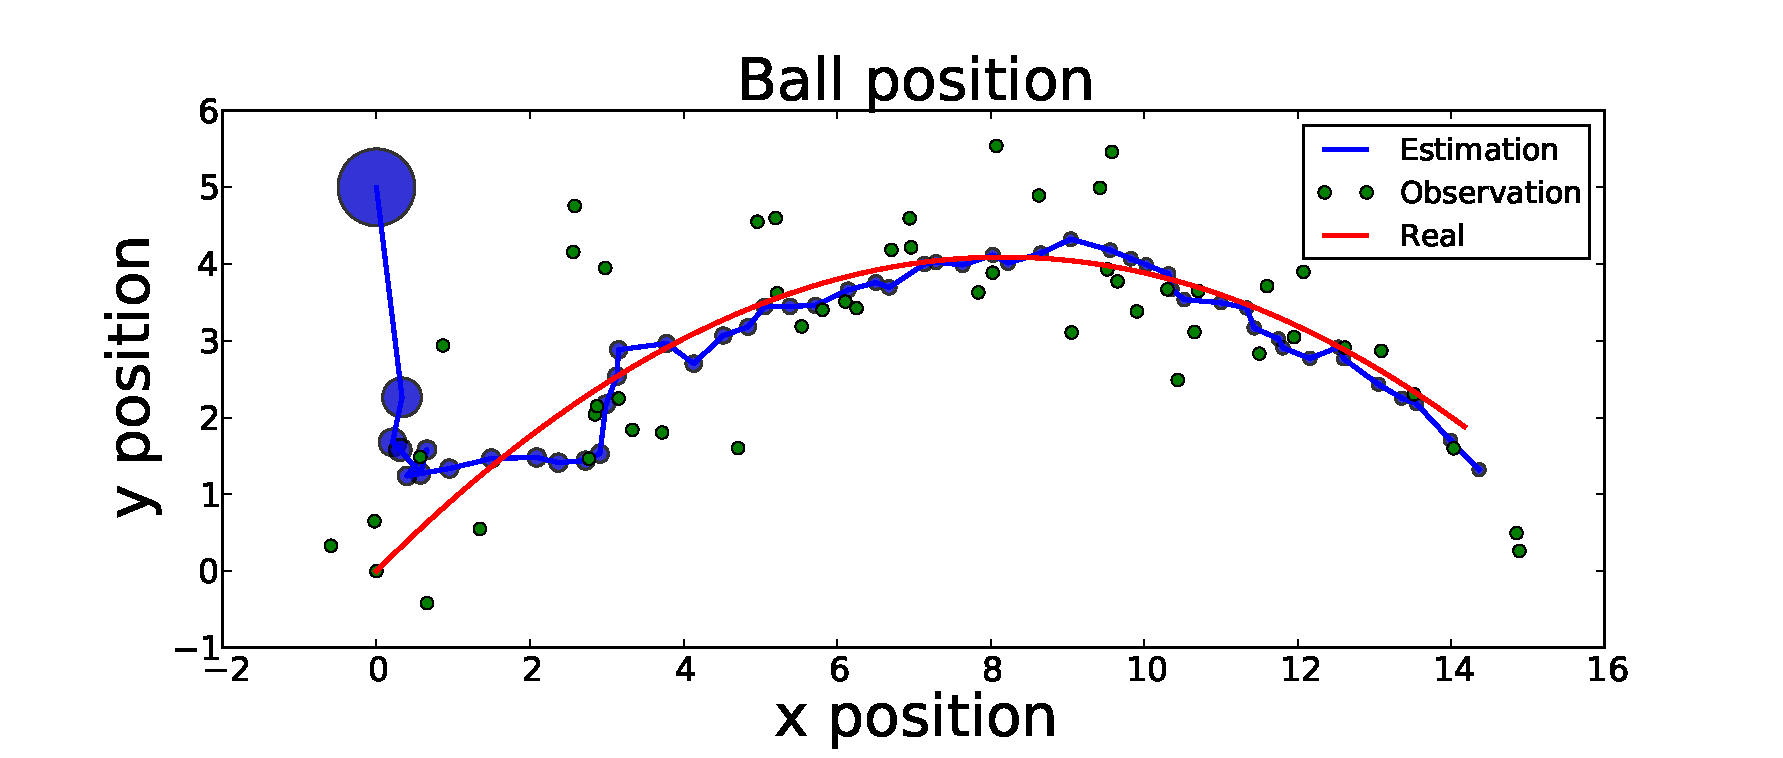
\includegraphics[width=0.8\linewidth]{Examples/KF-Ex/KF-ex1.pdf}
  \caption{\label{fig:KF-ex1} Simulation of a Kalman filter trying to
    estimate the trajectory of a ball launched with an initially
    unknown position and velocity.}
\end{figure}


\pagebreak

\section{EKF : using the jacobian to linearize a state-space formulation}
\subsection{Introduction}
The Extended Kalman Filter can be applied to estimate the state of a system $x_k$ given observations $y^\star_k$. The evolution function $f$ characterizing the evolution of the system's state and the observation function $h$ linking the state to the observations can be non-linear. However, EKF requires to compute the gradient of these functions relative to the state. EKF relies on a linearisation of the evolution and observation functions which are good approximations of the original functions if these functions are close to linear. The state-space formulation of EKF reads :
\begin{eqnarray}
\nonumber \vecteur{x}_{k} &=& f(\vecteur{x_{k-1}}) + \vecteur{w_{k}}\\
\label{eq_ekf} \vecteur{y_{k}} &=& h(\vecteur{x_k}) + \vecteur{v_k}
\end{eqnarray}
where $w$ and $v$ are independent white noises. As always with Kalman
filters, we look for the optimal gain $K_k$ (the so-called Kalman
gain) which updates an a priori estimate of the state $\hat{x}^-_k$
into an a posteriori estimate $\hat{x}_k$, minimizing the error
between this a posteriori estimate and the the real state, given the
observations. This can be done recursively given an a priori on the
covariance of the error. A standard Kalman filter considers $f$ and
$h$ to be linear (the evolution function is written $x_{k+1} = F x_{k}
+ w_k$, the observation function is written $y_{k} = H x_k + v_k$,
$F,H$ being matrices). Given this assumption, one can derive
analytically the Kalman gain and get an update of the shape $\hat{x}_k
= \hat{x}^-_k + K_k (y_k - H.\hat{x}^-_k)$. Non-linear evolution and
observation functions are handled within EKF by linearising these
functions around some estimates of the state; for example for the
evolution function is linearized around the previous estimate of the
state $\hat{x}_k$: $f(x_k) \approx f(\hat{x}_k) + \frac{\partial f}{dx}(\hat{x}_k) (x_k - \hat{x}_k)$. A standard Kalman filter can be applied on a new state-space formulation which is a linearisation of equations (\ref{eq_ekf}).\\

We start EKF with an estimate of the state $\hat{\vecteur{x}}_{0}$ and an associated
uncertainty $\matrice{P_0}$. The first step in applying EKF is to
linearize the evolution function around the previous estimate of the
state $\hat{\vecteur{x}}_{k-1}$ :
\begin{eqnarray}
\nonumber \vecteur{x}_{k} &\approx& f(\hat{\vecteur{x}}_{k-1}) +
\matrice{F}_{k-1} (\vecteur{x_{k-1}} - \hat{\vecteur{x}}_{k-1}) +
\vecteur{w_{k}}\\
&=& \matrice{F}_{k-1} \vecteur{x}_{k-1} + (f(\hat{\vecteur{x}}_{k-1}) -
\matrice{F}_{k-1}  \hat{\vecteur{x}}_{k-1}) + \vecteur{w}_{k} \\
\label{eq_ekf_linear_evolution}&=& \matrice{F}_{k-1} \vecteur{x}_{k-1} + \vecteur{u}_k + \vecteur{w}_{k}
\end{eqnarray}

where $\matrice{F}_{k-1}$ is the Jacobian of the evolution function taken in $\hat{\vecteur{x}}_{k-1}$ : 
\begin{eqnarray}
\matrice{F}_{k-1} &=& \begin{bmatrix}
\frac{\partial f_1}{\partial x_1}(\vecteur{x}) & \cdots & \frac{\partial f_1}{\partial x_n}(\vecteur{x})\\
\vdots & \ddots & \vdots\\
\frac{\partial f_n}{\partial x_1}(\vecteur{x}) & \cdots & \frac{\partial f_n}{\partial x_n}(\vecteur{x})
\end{bmatrix}_{\vecteur{x} = \hat{\vecteur{x}}_{k-1}} 
\end{eqnarray}

In equation (\ref{eq_ekf_linear_evolution}) we recognize a linear
evolution function for which we can apply the prediction step of
Kalman filtering on linear state space equations. Therefore, we get
the following prediction and associated covariance :
\begin{eqnarray}
\hat{\vecteur{x}}_k^-&=& \matrice{F}_{k-1}\hat{\vecteur{x}}_{k-1} +
( f(\hat{\vecteur{x}}_{k-1}) - \matrice{F}_{k-1}
\hat{\vecteur{x}}_{k-1}) =  f(\hat{\vecteur{x}}_{k-1})
\\
\matrice{P}_k^- &=& \matrice{F}_{k-1} \matrice{P}_{k-1}
\matrice{F}_{k-1}^T + \matrice{Q}_k
\end{eqnarray}

For the correction step, we first linearize the observation function
around the estimate of the state $\hat{\vecteur{x}}_k^-$ :
\begin{eqnarray}
\label{eq_ekf_linear_observation} \vecteur{y_{k}} &\approx&
h(\hat{\vecteur{x}}_k^-) + \matrice{H}_k .(\vecteur{x_{k}} -
\hat{\vecteur{x}}_k^-) + \vecteur{v_k}\\
&=& \matrice{H}_k \vecteur{x}_k + (h(\hat{\vecteur{x}}_k^-)-
\matrice{H}_k \hat{\vecteur{x}}_k^-) + \vecteur{v}_k\\
\vecteur{y_{k}} - (h(\hat{\vecteur{x}}_k^-)-
\matrice{H}_k \hat{\vecteur{x}}_k^-) \approx  \matrice{H}_k
.(\vecteur{x_{k}} + \vecteur{v}_k
\end{eqnarray}
where $\matrice{H}_k$ is the Jacobian of the observation function
taken in $\hat{\vecteur{x}}_k^-$ :
\begin{eqnarray}
\matrice{H}_{k} &=& \begin{bmatrix}
\frac{\partial h_1}{\partial x_1}(\vecteur{x}) & \cdots & \frac{\partial h_1}{\partial x_n}(\vecteur{x})\\
\vdots & \ddots & \vdots\\
\frac{\partial h_n}{\partial x_1}(\vecteur{x}) & \cdots & \frac{\partial h_n}{\partial x_n}(\vecteur{x})
\end{bmatrix}_{\vecteur{x} = \hat{\vecteur{x}}_k^-}
\end{eqnarray}
We can now apply the correction step of kalman filters for linear
state space :
\begin{eqnarray}
\matrice{K}_k &=& \matrice{P}_k^- \matrice{H}_k^T (\matrice{H}_k
\matrice{P}_k^- \matrice{H}_k^T + \matrice{R}_k)^{-1} \\
\matrice{P}_k &=& (\matrice{I} - \matrice{K}_k \matrice{H}_k)
\matrice{P}_k^- \\
\nonumber \hat{\vecteur{x}}_k &=& \hat{\vecteur{x}}_k^- + \matrice{K}_k
(\vecteur{y_{k}} - (h(\hat{\vecteur{x}}_k^-)- \matrice{H}_k
\hat{\vecteur{x}}_k^-) - \matrice{H}_k \hat{\vecteur{x}}_k^-)\\
&=&  \hat{\vecteur{x}}_k^- + \matrice{K}_k (\vecteur{y_{k}} - h(\hat{\vecteur{x}}_k^-))
\end{eqnarray}

\subsection{Summary}

In summary, given an a priori estimate $\hat{\vecteur{x}}_0$ of the
state and its associated covariance (uncertainty) $\matrice{P}_0$, the
equations of Extended Kalman filtering are the following :\\
\textbf{State-space formulation :}\\
\begin{eqnarray}
\vecteur{x_k} &=& f(\vecteur{x}_{k-1}) + \vecteur{w}_{k}\\
\vecteur{y_k} &=& h(\vecteur{x_k}) + \vecteur{v_k}
\end{eqnarray}
with $w_k\sim N(0,Q_k), v_k \sim N(0,R_k)$.\\
\textbf{Prediction step:}\\
\begin{eqnarray}
\hat{\vecteur{x}}^-_k &=& f(\hat{\vecteur{x}}_{k-1})\\
\matrice{P^-_k} &=& \matrice{F}_{k-1} \matrice{P_{k-1}} \matrice{F}_{k-1}^T + \matrice{Q_k}
\end{eqnarray}
\textbf{Correction step:}\\
\begin{eqnarray}
\matrice{K_k} &=& \matrice{P^-_k} \matrice{H}_k^T . (\matrice{H}_k \matrice{P^-_k} \matrice{H}_k^T +\matrice{R_k})^{-1}\\
\matrice{P_k} &=& (\matrice{I} - \matrice{K_k} \matrice{H}_k) \matrice{P^-_k}\\
\hat{\vecteur{x}}_k &=& \hat{\vecteur{x}}^-_k + \matrice{K_k} (\vecteur{y_k} - h(\hat{\vecteur{x}}_k^-))
\end{eqnarray}
with the following definitions of $\matrice{F}_{k-1}$ and $\matrice{H}_k$ :
\begin{eqnarray}
\matrice{F}_{k-1} &=& \begin{bmatrix}
\frac{\partial f_1}{\partial x_1}(\vecteur{x}) & \cdots & \frac{\partial f_1}{\partial x_n}(\vecteur{x})\\
\vdots & \ddots & \vdots\\
\frac{\partial f_n}{\partial x_1}(\vecteur{x}) & \cdots & \frac{\partial f_n}{\partial x_n}(\vecteur{x})
\end{bmatrix}_{\vecteur{x} = \hat{\vecteur{x}}_{k-1}} \\
\matrice{H}_{k} &=& \begin{bmatrix}
\frac{\partial h_1}{\partial x_1}(\vecteur{x}) & \cdots & \frac{\partial h_1}{\partial x_n}(\vecteur{x})\\
\vdots & \ddots & \vdots\\
\frac{\partial h_n}{\partial x_1}(\vecteur{x}) & \cdots & \frac{\partial h_n}{\partial x_n}(\vecteur{x})
\end{bmatrix}_{\vecteur{x} = \hat{\vecteur{x}}_k^-}
\end{eqnarray}

\subsection{Examples}

We can now handle non-linear evolution and observation functions. We
first consider an example of this ability. Let's consider the following dynamical system :
\begin{eqnarray}
\dot{x}(t) &=& \frac{2.0}{1 + exp(-(y(t)-1))} -1.0\\
\dot{y}(t) &=& -k*x(t)\\
\begin{bmatrix}
\dot{x}(t) \\
\dot{y}(t)
\end{bmatrix} &=& F(\begin{bmatrix}
x(t) \\
y(t)
\end{bmatrix}) \\
x(0) = 1.0 \\
y(0) = 0.0 
\end{eqnarray}
The evolution of $x(t)$ depends non-linearly on $y(t)$, through a
sigmoid which may introduce weak or strong non-linearity in the
evolution function depending on the value of $k$ which increases the
range of evolution of $y(t)$ and ultimately impacts on whether or not
the sigmoid is applied in its linear or non-linear range. The fig
\ref{fig:ekf_ex1_simu}a shows a plot of the above sigmoid. Roughly
speaking, if we are in the range $[-3;3]$ the sigmoid is linear and it
becomes non-linear out of this range. The figure \ref{fig:ekf_ex1_simu}b shows a simulation of this system. It is in
the rising phase of $y(t)$ that the evolution function becomes
non-linear. We will apply EKF to see how it behaves in this situation
compared to situation where the evolution function is linear. The
dynamical system is updated with a forward Euler method which keeps
the evolution function simple but forces us to use a very small time
step, here of $5e^{-4} s.$.\\

%\footnote{Given a dynamical system defined as $\dot{X}(t) = f(t,
%X(t))$, the RK4 method computes a new $X(t_k)$ from a previous state
%$X(t_k + \delta t)$ as $X(t_k + \delta t) = X(t_k) + \frac{\delta
%t}{6}(k_1 + 2 k_2 + 2k_3 + k_4)$ with $k_1 = f(t_k, X(t_k))$, $k_2=
%f(t_k + \delta t/2, X(t_k) + \delta t/2 k_1)$, $k_3 = f(t_k + \delta
%t/2, X(t_k) + \delta t/2 k_2)$ and $k_4 = f(t_k + \delta t, X(t_k) + \delta t k_3)$.}

\begin{figure}
\begin{center}
\begin{tabular}{cc}
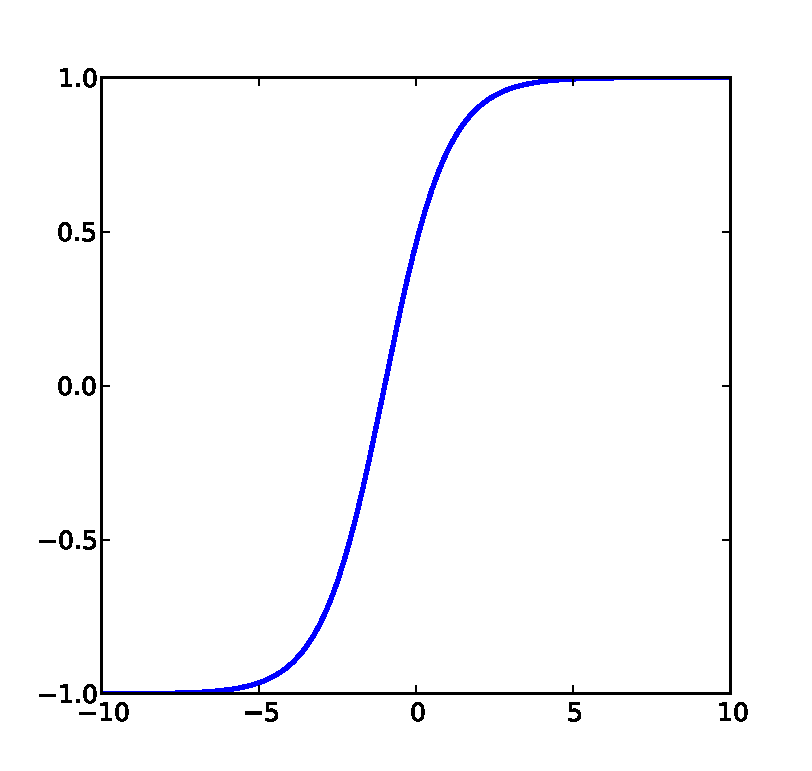
\includegraphics[height=5cm]{Examples/EKF-Ex/plot_sigmoid.pdf} &
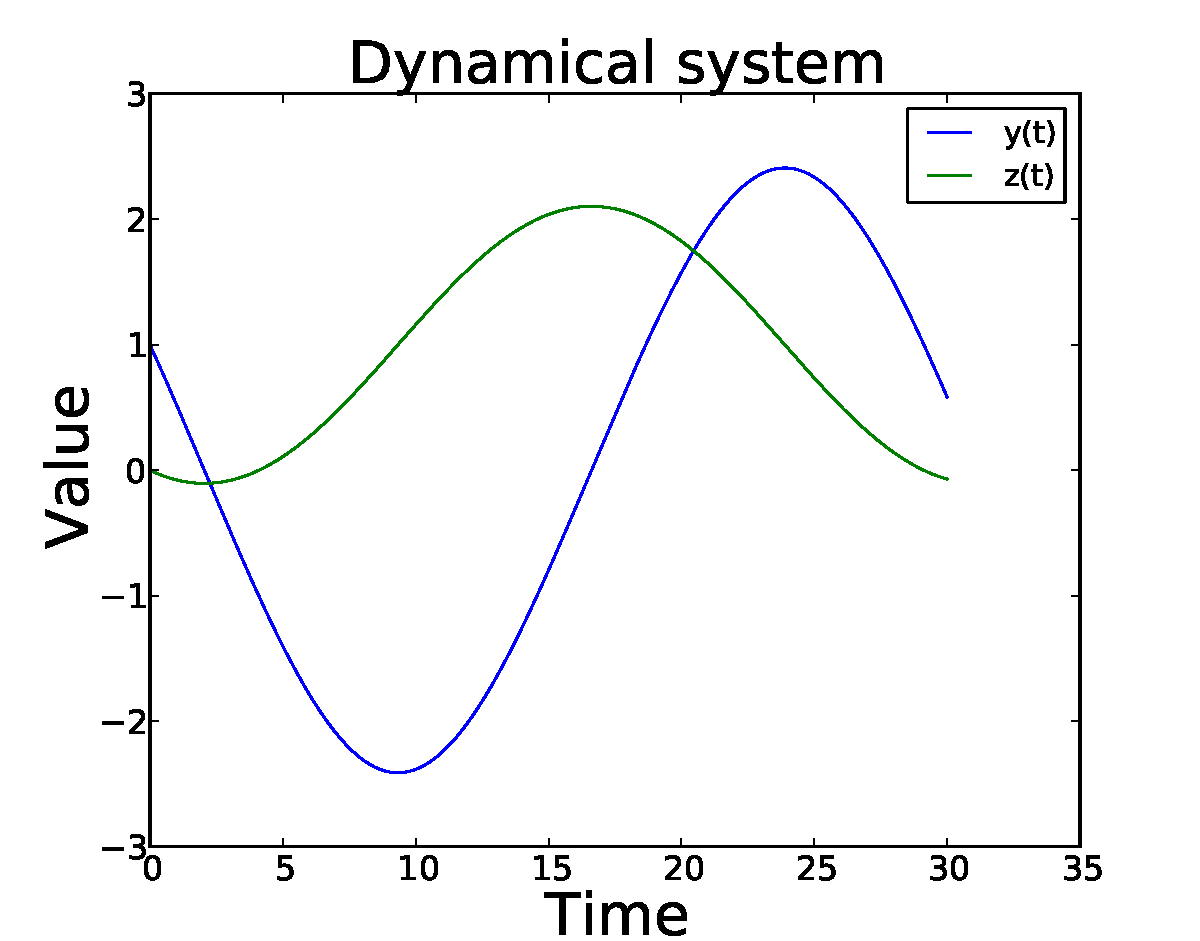
\includegraphics[height=5cm]{Examples/EKF-Ex/simulation_ex1.pdf}\\
a) & b)
\end{tabular}
\end{center}
\caption{\label{fig:ekf_ex1_simu} a) The transfer function is a sigmoid,
  almost linear in the xrange $[-3;3]$ and highly non-linear outside
  of this range. b) The simulated system is oscillatory. Depending on
  the factor $k$, the system may have phases where $y(t)$ enters the
  non-linear range of the sigmoid and other phases where the evolution
  function can be well linearly approximated.}
\end{figure}

In order to use EKF, we need to define the state-space
formulation. Using a forward Euler scheme, the state-space formulation reads :
\begin{eqnarray}
\nonumber \begin{bmatrix}
x_k \\
y_k
\end{bmatrix} &=& f( \begin{bmatrix}
x_{k-1} \\
y_{k-1}
\end{bmatrix}) + \vecteur{w}_k \\
\nonumber  &=& \begin{bmatrix}
x_{k-1} \\
y_{k-1}
\end{bmatrix} + \delta t F(\begin{bmatrix}
x_{k-1} \\
y_{k-1}
\end{bmatrix})\\
\vecteur{z}_k &=& h( \begin{bmatrix}
x_{k} \\
y_{k}
\end{bmatrix}) + \vecteur{v}_k = \begin{bmatrix}
x_{k} \\
y_{k}
\end{bmatrix} + \vecteur{v}_k
\end{eqnarray}
For the simulations, we used $\delta t = 5.10^{-4}$. The results of applying EKF
to estimate the state $(y(t),z(t))$ from noisy observations of the
real system are shown on fig \ref{fig:ekf_ex1}.

\begin{figure}
\center 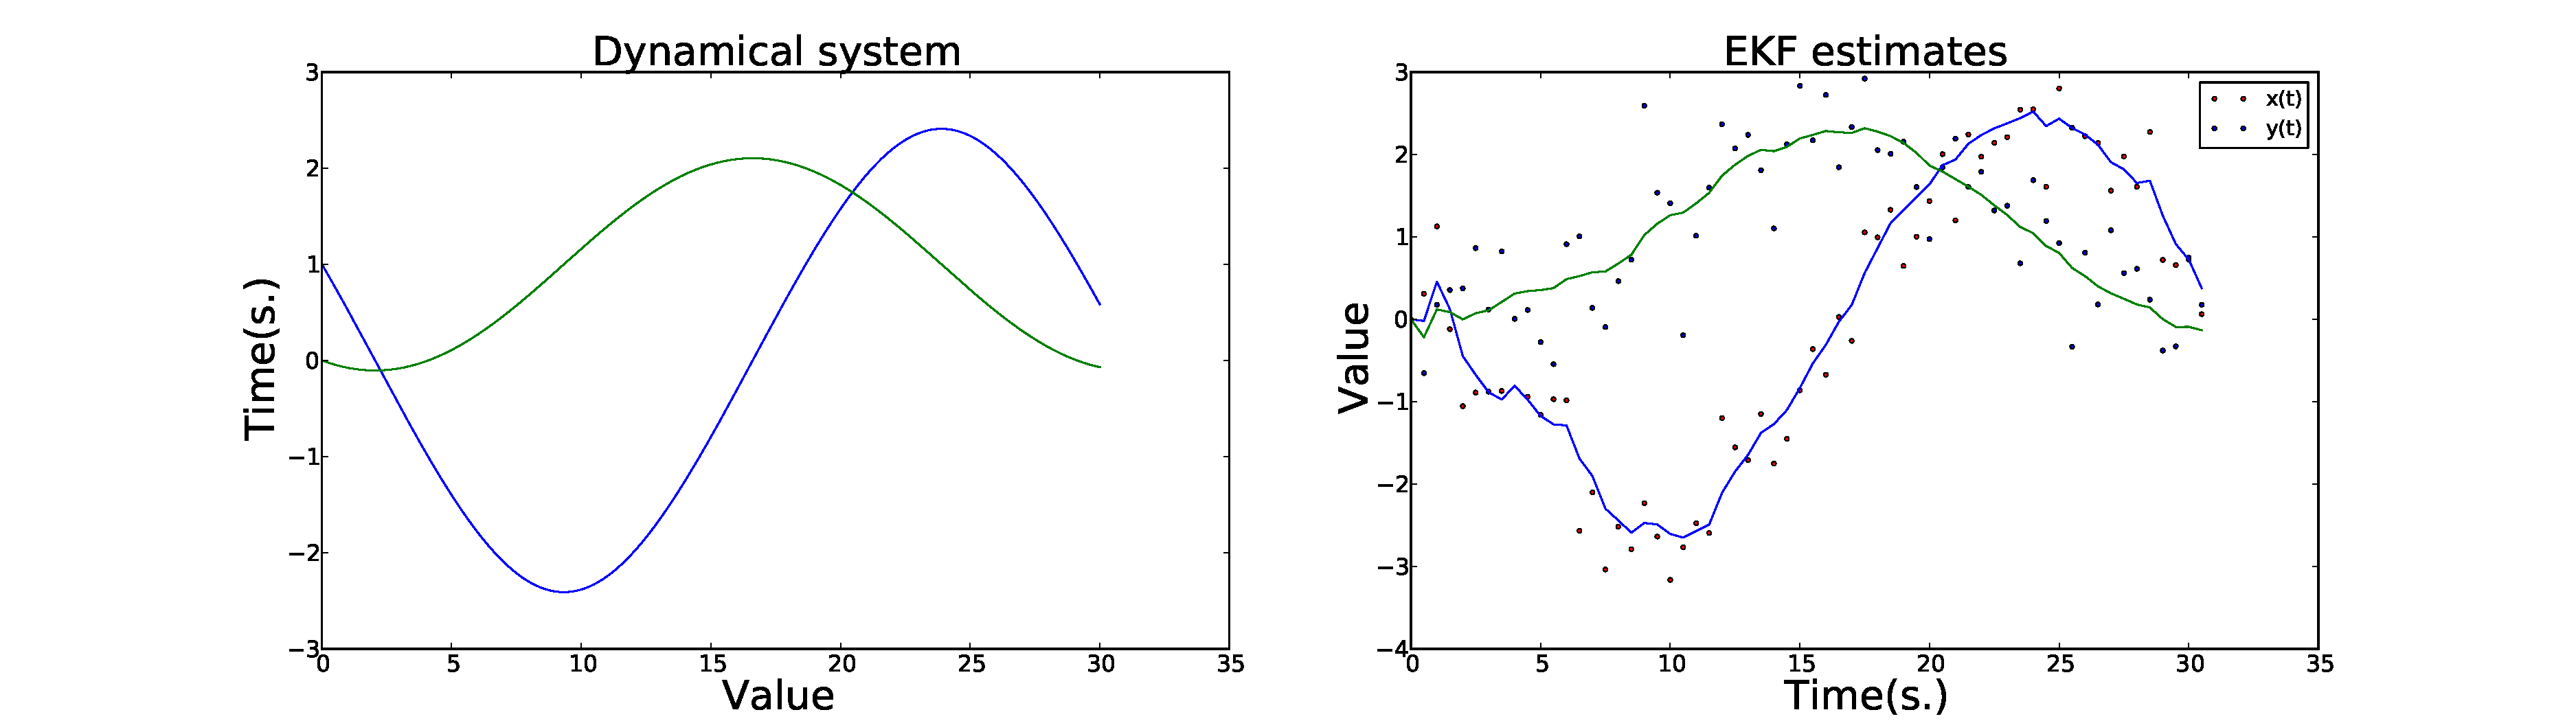
\includegraphics[width=0.9\linewidth]{Examples/EKF-Ex/EKF-ex1.pdf}
\caption{\label{fig:ekf_ex1} Application of EKF to estimate the state
  of a non-linear dynamical system.}
\end{figure}

%% The algorithm of EKF is the algorithm \ref{algo_ekf}

%% \begin{algorithm}
%% \caption{The extended kalman filter, estimating $n$ parameters}
%% \label{algo_ekf}
%% \begin{algorithmic}
%% \STATE \textbf{0 - Initialization}
%% \end{algorithmic}
%% \end{algorithm}

\vfill
\pagebreak

\section{UKF : estimating an arbitrary non-linear transformation of a random variable}

\textcolor{red}{TODO ....}\\

As we saw in the previous section, the Extended Kalman Filter deals
with non-linear evolution and observation functions by approximating
them at the first order. It also requires to be able to compute the
jacobian of these functions. This leads to two flaws of EKF :
approximation errors when the evolution and observation functions are
not locally linear and the inability of EKF to handle non-derivable
functions. The Unscented Kalman Filter is another approach for
handling non-linear evolution and observation functions. It relies on
the idea that it is easier to approximate any non-linear
transformation of a random variable than to approximate arbitrary
non-linear functions (as done with the Jacobian in EKF)
\cite{Julier2004}. A thorough presentation of the unscented kalman filter algorithms can be found in \cite{Merwe2004}.

\subsection{Introduction}

The Unscented Kalman Filter relies on the Unscented Transform which
tries to solve the following problem\~: \emph{Let $x$ be a random variable
  with mean $\bar{x}$ and covariance $\matrice{P}_{xx}$. A second
  random variable $y$ related to $x$ as $y = f(x)$ is introduced. We wish to calculte the first two moments of $y$ : its mean $\bar{y}$ and covariance $\matrice{P}_{yy}$}.\\

For this problem, three desired properties are introduced :
\begin{itemize}
\item consistency : $\matrice{P}_{yy} - E[(y-\bar{y}).(y-\bar{y})^T]
  \geq 0$
\item efficiency : $\matrice{P}_{yy} - E[(y-\bar{y}).(y-\bar{y})^T]$
  must be minimized
\item unbiased : $\bar{y} \approx E[y]$
\end{itemize}

Consistency means that the covariance of $y$ is never under
estimated. This is an important feature of Kalman filters. If the
covariance is underestimated, the resulting kalman filter may be
diverging. A consistent, efficient and unbiased transformation
procedure can be examined by considering the Taylor series expansion
of the expression of $y$ around $\bar{x}$ \cite{Julier1997}.\\


\subsection{The Unscented Transform}

\textcolor{red}{La UT pourrait être utiliser pour estimer comment
  l'incertitude sur les valeurs des paramètres d'un modèle se
  propagent sur l'incertitude des réponses}


 It relies on the Unscented Transform schematically depicted on figure \ref{fig:UT}.\\

\begin{figure}[htbp]
\begin{center}
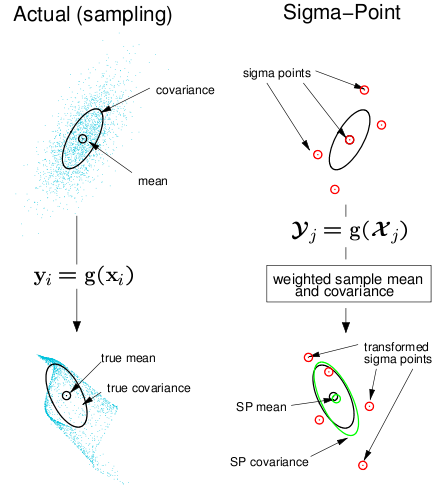
\includegraphics[width=0.3\linewidth]{eps/UT2.png}
\end{center}
\caption{\label{fig:UT} Illustration of the Unscented Transform}
\end{figure}

The problem that the unscented transform seeks to solve is to estimate the mean and variance of a non-linear transformation of a random variable. Starting with a random variable $X$ of mean $\bar{X}$ and covariance $\Sigma_X$, we start by defining a set of $2n+1$ sigma points $X_j$ (where $n$ is the number of components of $X$). These sigma-points are defined such that their mean and covariance are the same than the random variable $X$, namely :
\begin{eqnarray}
\overline{X} &=& \frac{1}{2n+1} \sum_j X_j \\
\Sigma_X &=& \frac{1}{2n+1} \sum_j (X_j - \overline{X})(X_j - \overline{X})^T
\end{eqnarray}
 Then we compute the image, denoted $Y_j = g(X_j)$, of these $2n+1$ sigma-points through the non-linear transformation. We now introduce a set of $2n+1$ weights $W_j$ such that the weighted mean and covariance of the images is as close as possible to the true mean and covariance of the transformed random variable :
\begin{eqnarray}
\overline{g(X)} &\approx& \overline{Y} = \frac{1}{2n+1} \sum_j W_j Y_j\\
\Sigma_{g(X)} &\approx& \Sigma_Y = \frac{1}{2n+1} W_j (Y_j - \overline{Y})(Y_j - \overline{Y})^T
\end{eqnarray}
Now the question remains on how to define the sigma-points $X_j$ and which
values should we use for the weights $W_j$.

\subsection{UKF for parameter estimation}

\subsection{UKF for state estimation}

\subsection{Dual estimation}


\bibliographystyle{apalike}
%\bibliographystyle{plain}
\bibliography{biblio}

\end{document}
